\chapter{安全分析手法STAMP/STPA}
%岡本さん
\label{chap3}

\section{STAMPの概要}

% pp.6-8の「背景」は(今は)書かないことにする。
STAMP(System-Theoretic Accident Model and Processes)は、システム理論に基づく新しい事故モデル(Accident Model)です。
従来の事故モデルが主にコンポーネントと呼ばれるシステムの構成要素の故障(Failure)に焦点を当てているのに対し、STAMPはシステム全体の安全制約とその制御に注目します。

% \subsection{STAMPの基本概念}

STAMPの基本要素は以下の3つです: % pp.11
%
\begin{itemize}
    \item 安全制約(Safety Constraint):安全が守られるためにシステムやコンポーネントが守る必要があるルール。
    \item プロセスモデル(Process Model):コントローラが認識するコントロール対象の状態。
    \item 安全制御構造(Safety Control Structure):コンポーネントとそれらの間の相互作用(制御関係とフィードバック関係)を機能レベルで表したシステムのモデル。
\end{itemize}
%
STAMPでは、事故を単純なイベントの連鎖ではなく、安全制約が安全制御により適切に守られなかった結果として捉えます。

%%%%%%%%%%%%%%%%%%%%%%%%%%%%%%%%%%%%%%%%%%%%%%%%%%%%
\section{STPA}

STPA(System-Theoretic Process Analysis)は、STAMPに基づくハザード分析手法です。
システムの設計段階や運用開始前に潜在的なハザードを特定し、安全制約を導出するために使用されます。

%%%%%%%%%%%%%%%%%%%%%%%%%%%%%%%%%%%%%%%%%%%%%%%%%%%%
\subsection{STPAの手順}

STPAは以下の4つのステップで構成されます(STPA Handbook(2018)):
%
\begin{itemize}
    \item Step 1: 分析目的の定義
    \item Step 2: 安全制御構造図(Safety Control Structure Diagram)のモデル化
    \item Step 3: 非安全制御動作(Unsafe Control Action)の識別
    \item Step 4: ロスシナリオ(Loss Scenario)の識別
\end{itemize}
%
以下の各項で、STPAの各ステップについて解説します。

%%%%%%%%%%%%%%%%%%%%%%%%%%%%%%%%%%%%%%%%%%%%%%%%%%%%%%%%%%%%%%%%
\subsection{Step 1: 分析目的の定義}

Step 1「分析目的の定義」では、以下を項目を実施します: %pp.27
%
\begin{itemize}
    \item ロスの識別
    \item システムレベルのハザードの識別
    \item システムレベルの安全制約の識別
    \item ハザードの詳細化(任意)
\end{itemize}
%
各項目について解説します。 % pp.28

ロス(Loss)は、ステークホルダにとって受容できない何かを表します。
ロスの例としては、人命の喪失、人の負傷、環境汚染、ミッション失敗等が挙げられます。
以前のSTPAの解説ではアクシデント(Accident)も識別されていましたが、STPA Handbook(2018)からは、アクシデントを識別するよう記載されていません。
しかし、ロスと合わせてアクシデントを識別することで、後述するハザードが識別しやすくなるため、ここではアクシデントについても触れることにします。
アクシデントは、望まれない・計画されていないイベントで、ロスへ至るものです。
アクシデントの例として、自車両が前方障害物に激突等が挙げられます。

システムレベルのハザード(Hazard)は、システムの状態または条件の集まりで、最悪の環境条件下で、ロスへ至る蓋然性が高いものです。
ハザードはシステムの状態または条件の集まりであるため、システム境界外の状態または条件の集まりを直接は扱えません。
例えば、「自車両が(外部環境である)前方障害物に衝突した状態」はハザードではありません。
この場合、例えば「(自車両内の前方障害物検出用の)距離センサの値が規定値未満である状態」をハザードとします。
また、ハザードは必ずしもロスへ至るわけではない点にも、注意が必要です。
例えば、距離センサの値が規定値未満であったとしても、運転者の回避能力が高い場合には前方障害物を回避でき、人命の喪失や負傷へ至らないかもしれません。
さらに、自動車である以上不可避な状態である「自車両が走行中である状態」も、最悪の環境下でロスへ至りますが、ロスへ至る蓋然性が低い(ロスに至るまでの追加条件が多い)ため、ハザードしては扱いません。

システムレベルの安全制約は、システムレベルの条件・動作で、ハザードを防ぐためにシステムが満たす必要のあるものです。
素朴な安全制約はハザードの裏返しとして定義でき、またハザード発生時にロスを防ぐあるいは最小化する条件・動作としても定義できます。
例えば、自動運転システムを開発・分析しているときには、ハザード「距離センサの値が規定値未満である状態」を防止するために、
「自動運転システムは、距離センサの値が規定値未満になったら、自車両を安全に停止させなければならない」
といった安全制約が考えられます。

\textcolor{red}{ハザードの詳細化(任意)では、…}

一般に、多数のロス、ハザード、安全制約が識別されるため、
ロス、ハザード、安全制約は、番号を付け、ハザードには対応するロスの番号を含めることで、
分析結果の整理が容易になります。

%%%%%%%%%%%%%%%%%%%%%%%%%%%%%%%%%
\subsubsection{演習:ロス、ハザード、安全制約の識別} % pp.29-35

\textcolor{red}{システムの説明を記述し、図を挿入すること。}

\begin{enumerate}
    \item 上のシステムに対するロス及びアクシデントを識別しなさい。
    (解答例:乗員の死亡・負傷(自車両が前方障害物に衝突))
    \item (i)で識別したロスに対し、ハザードを識別しなさい。
    (解答例:(前方障害物検出用の)距離センサの値が規定値未満)
    \item (ii)で識別したハザードに対し、安全制約を識別しなさい。
    (解答例1:距離センサの値が規定値未満になってはならない。解答例2:自動ブレーキシステムは、距離センサの値が規定値未満にならないよう、ブレーキを指示しなければならない。)
\end{enumerate}

%%%%%%%%%%%%%%%%%%%%%%%%%%%%%%%%%%%%%%%%%%%%%%%%%%%%%%%%%%%%%%%%
\subsection{Step 2: 安全制御構造図のモデル化}

Step 2「安全制御構造図のモデル化」では、安全制御構造図を構築します。
安全制御構造図は、システム内の構成要素(コンポーネント)間の制御関係とフィードバック関係を示すシステムのモデルで、
コントロール・ループ(図3.1)により構成されます。
ここで、コントロール・ループは以下の構成要素により構成されます。
%
\begin{itemize}
    \item コントローラ:制御する側のコンポーネント。
    \item コントロールアルゴリズム:コントローラの判断決定プロセス。コントローラは、コントロールアルゴリズムに基づき、コントロールアクションを指示します。
    \item プロセスモデル:コントローラの内部情報で、判断の際に参照される情報。プロセスモデルは、コントローラが認識する被コントロール・プロセスや外部環境の状態であり、フィードバックにより更新されます。
    \item 被コントロール・プロセス:制御される側のコンポーネント。
    \item コントロールアクション:被コントロール・プロセスの動作や制約を実行させるためのコントローラが出す命令・指示。
    \item フィードバック:被コントロール・プロセスや外部環境からコントローラに送られてくる情報。
\end{itemize}
%
\begin{figure}[H]
    \centering
    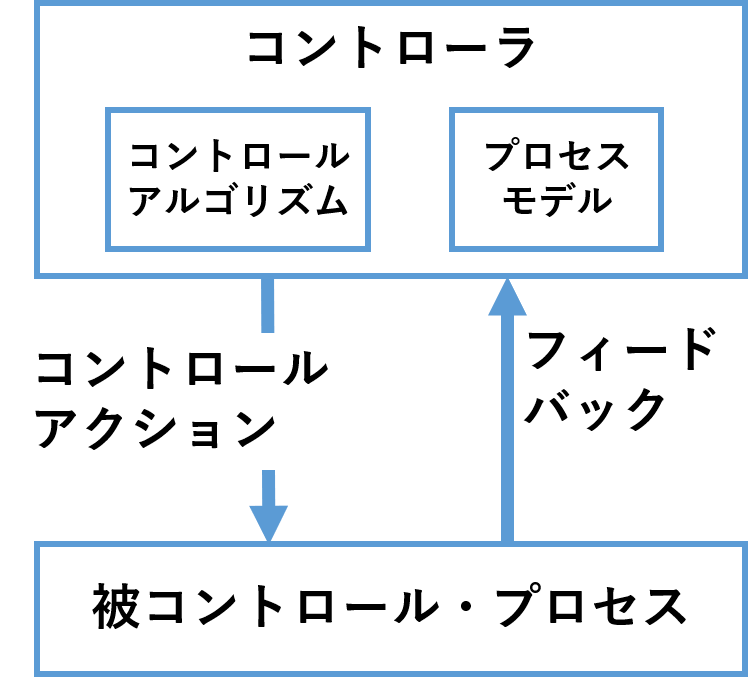
\includegraphics[width=80mm]{safety_assurance_contents/ch3images/fig-3-2-3-01.png}
    \caption{コントロール・ループ}
\end{figure}

図3.2は、赤線で囲まれた二つのコントロール・ループにより構成される安全制御構造図の例です。
安全制御構造図では、制御する側を上に、制御される側を下にして記述します。
また図3.2には、アクチュエータとセンサを記載してありますが、比較的新しい文献では、
安全制御構造図を構築する際にはこれらを記載せず、後の分析(Step4)でこれらを追加して分析をするようになっています。

\begin{figure}[H]
    \centering
    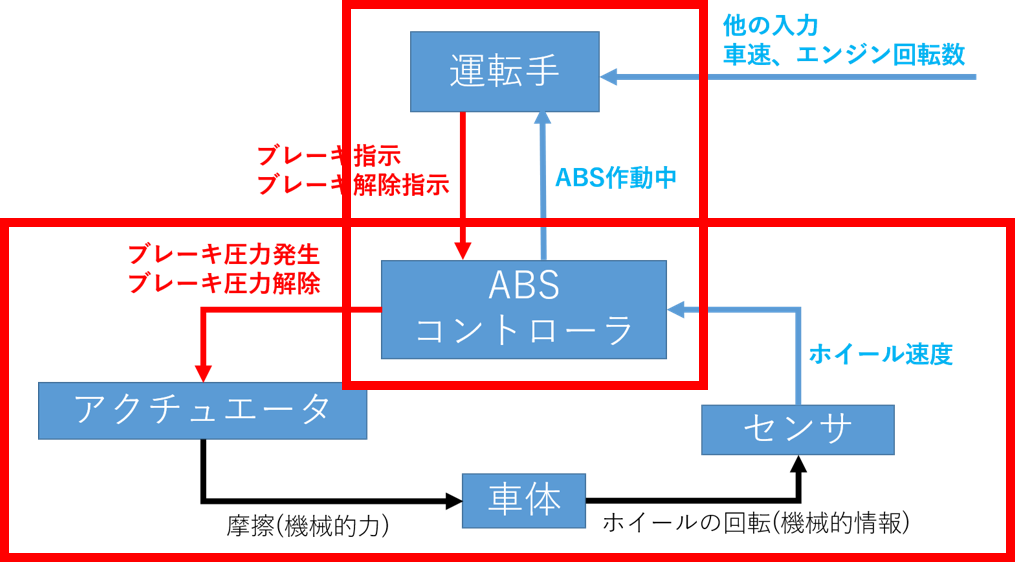
\includegraphics[width=80mm]{safety_assurance_contents/ch3images/fig-3-2-3-02.png}
    \caption[short]{例:二つのコントロール・ループにより構成される安全制御構造図}
\end{figure}

安全制御構造図は、物理的設計レベルではなく、機能レベルでのシステムのモデルです。
また、安全制御構造図はモデルですので、安全機構に関係無い機能は省略します。

安全制御構造図を基に分析することで、例えば、
センサが故障した結果、コントローラが間違ったフィードバックを受信して、
コントローラが誤った判断を下すといった事故のシナリオが識別できます。
また、プロセスモデルを考えることで、実際は自車両の前方に歩行者がいるのに、
コントローラ(自動運転車)は歩行者がいないと認識しており、その結果、事故に至るといったシナリオを分析しやすくなります。
さらに、コントローラが判断する際に必要なフィードバックが不足していたといった重大な欠陥を早期に見つけやすくなります。

機械以外にも、人間や組織をコントローラとする場合もあります。
この場合、コントロールアルゴリズムは人間の判断プロセスに、プロセスモデルは人間の認識になります。
また、(分析対象システムの外側である)外部環境からのフィードバックを考えることもあります。
例えば、自動運転車の安全制御構造図では、運転者を最上位のコントローラとし、運転者へのフィードバックとして、
目視情報(自車両の前方に歩行者がいる・いない等)を考えます。
分析の際に、安全制御構造図に人間や組織を含められるため、人間のミスや、他組織からの外圧を含めた事故のシナリオを考えられるようになります。

%%%%%%%%%%%%%%%%%%%%%%%%%%%%%%%%%%%%%%%%%%%%%%%%%%%%%%
\subsubsection{演習:安全制御構造図の構築} % pp.44

\textcolor{red}{システムの説明を記述し、図を挿入すること。}

%% pp.52-66の「詳細化によるCSDの構築」を書くか?

%%%%%%%%%%%%%%%%%%%%%%%%%%%%%%%%%%%%%%%%%%%%%%%%%%%%%%%%%%%%%%%%
\subsection{Step 3: 非安全制御動作の識別}

Step 3「非安全制御動作の識別」では、非安全制御動作(UCA: Unsafe Control Action)を識別し、可能であればコントローラ制約を定義します。
UCAは、特定のコンテキストと最悪の環境の下で、ハザードを引き起こす可能性のある制御動作で、
コントローラ制約はUCAを引き起こさないために満たす必要のあるコントローラへの動作(制約)です。

UCAは文章として表すことが多いですが、

「制御動作を出すコントローラ」+「タイプ」+「制御動作」+「コンテキスト」+「ハザード」

の組として考えると、UCAを識別しやすくなります。
このとき、タイプとして以下の4つを用います:
%
\begin{enumerate}
    \item 与えられないとハザード
    \item 与えられるとハザード
    \item 早すぎ、遅すぎ、誤順序でハザード
    \item 早すぎる停止、長すぎる適用でハザード
\end{enumerate}
また、コンテキストは制御動作が非安全となる条件を表します。

UCAの例として、「運転者からのブレーキ指示があり、タイヤがロックしていないにもかかわらず、ABSコントローラがブレーキ圧力発生を指示しないため,前方障害物との距離が規定値未満になる.(H3)」を考えます。
コントローラ「ABSコントローラ」に対するこのUCA対するコントローラ制約として、このUCAを否定形である
「運転者からのブレーキ指示があり、タイヤがロックしていないときには、ABSコントローラがブレーキ圧力発生を指示する。」
を考えることができます。
このとき、このUCAは以下のように分解されます:
%
\begin{itemize}
    \item 制御動作を出すコントローラ:ABSコントローラ
    \item タイプ:与えない
    \item 制御動作:ブレーキ圧力発生
    \item コンテキスト:運転手からのブレーキ指示があり、タイヤがロックしていない
\end{itemize}
%
制御動作を出すコントローラ、タイプ、制御動作、ハザードは既に識別されているため、それらを組み合わせて考えることで、網羅的な分析が可能になります。
しがって、コンテキストを識別することが最も重要となります。
このとき、制御動作を出すコントローラの入力に着目すると、コンテキストが考えやすくなります。
また識別したUCAに番号を付け、以下のような表形式で表すと可読性が高まり、後の分析が容易になります。
%
\begin{figure}[H]
    \centering
    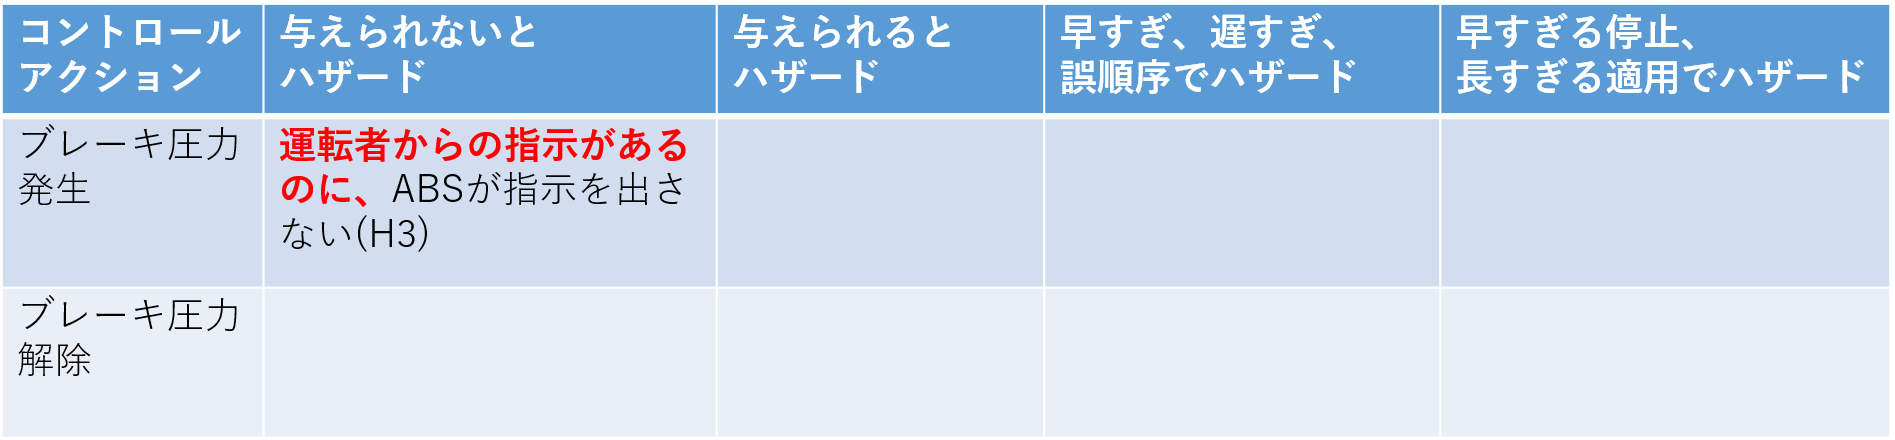
\includegraphics[width=100mm]{safety_assurance_contents/ch3images/fig-3-2-3-03.png}
    \caption[short]{例:UCAの表}
\end{figure}

コンテキストが無いにもかかわらずUCAとなる場合や、同じコンテキストの下で与えても、
与えなくてもUCAとなる場合には、その制御動作は設計には問題があると考えられます。

\subsubsection{演習:UCAの識別} % pp.74,75

\textcolor{red}{システムの説明を記述し、図を挿入すること。}

%%%%%%%%%%%%%%%%%%%%%%%%%%%%%%%%%%%%%%%%%%%%%%%%%%%%%%%%%%%%%%%%
\subsection{Step 4: ロスシナリオの識別}

Step 4「ロスシナリオの識別」では、Step 3で識別したUCAに対してロスシナリオを識別します。
ロスシナリオ(Loss Scenario)は、UCA、ひいてはハザードへ至る要因を記述したシナリオです。
ロスシナリオの中で具体的要因を識別するので、アクチュエータとセンサを入れたコントロール・ループを基に分析します。

大きく分けて、以下の2種類のロスシナリオを考えます:
%
\begin{itemize}
    \item UCAへ至るシナリオ
    \item 制御動作の不実行・不適切な実行を表すシナリオ
\end{itemize}
%
「UCAへ至るシナリオ」では、図3.2.5.1の右上部分に着目し、なぜUCAが発生したのかを考えます。
UCAが発生する一般的な要因としては、コントローラの非安全な動作や、不適切なフィードバック・(他コントローラ等からの)入力が考えられます。
% 84ページ「コントロールループで安全制約を破られる要因の例2」の図を入れるか?
また「制御動作の不実行・不適切な実行を表すシナリオ」では、図3.2.5.1の左下部分に着目し、
なぜ制御動作は不適切に実行されたのか、なぜ制御動作は実行されなかったのかを考えます。
「制御動作の不実行・不適切な実行が起こる一般的な要因としては、
アクチュエータやコントロールアクションの伝達経路上での問題、被コントロール・プロセスに関する要因が考えられます。
% 85ページ「コントロールループで安全制約を破られる要因の例3」の図を入れるか?
STPA Handbook(2018)やはじめてのSTAMP/STPA(2016)には、ロスシナリオを識別する際のヒントとして、一般的要因のリストが例示されています。
このような一般的要因や過去の知見から得られている独自要因のリストは、ロスシナリオの識別に有用です。
しかし、このようなリストを一通り考察したら分析を終えるのではなく、他の要因が無いかを検討することが肝要です。
%
\begin{figure}[H]
    \centering
    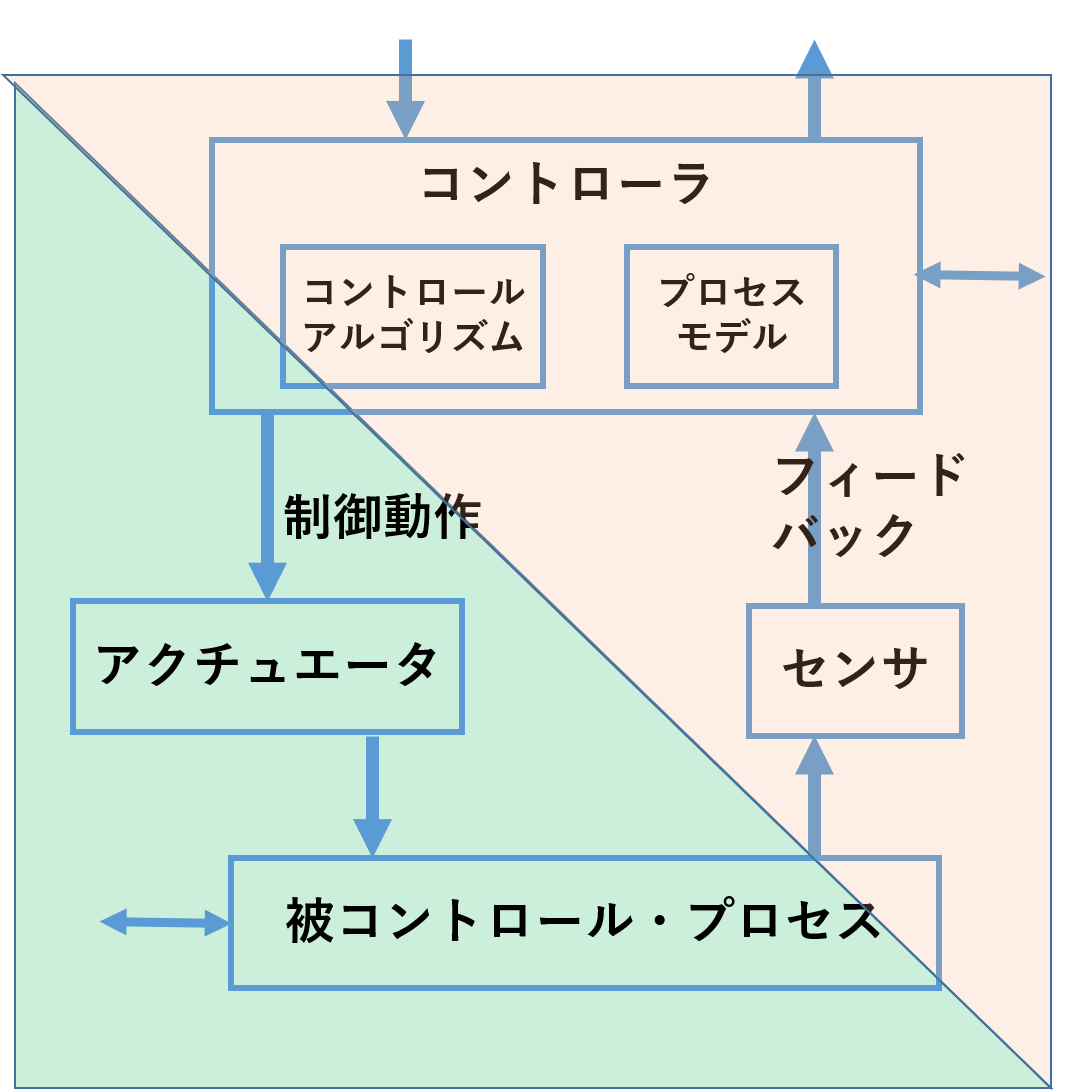
\includegraphics[width=80mm]{safety_assurance_contents/ch3images/fig-3-2-5-01.png}
    \caption[short]{考えるべきロスシナリオ}
\end{figure}

\textcolor{red}{(ハザードからロスシナリオまで一貫性・妥当性のある例に変更すること!)}
UCA「運転者からのブレーキ指示があり、タイヤがロックしていないにもかかわらず、ABSコントローラがブレーキ圧力発生を指示しないため,前方障害物との距離が規定値未満になる。」を考えます。
このUCAに対するロスシナリオ、特にUCAへ至るシナリオの例としては、
「センサからのフィードバックが間違っていたため、ABSコントローラがタイヤがロックしていないと誤認識してしまい、ABSコントローラがブレーキ圧力発生を指示しない。」が考えられます。
このように現実とプロセスモデル(コントローラの認識)が異なる状況は、プロセスモデルの不一致と呼ばれ、ロスシナリオを識別する際に、しばしば登場します。
また、制御動作の不実行・不適切な実行を表すシナリオの例としては、
「アクチュエータが故障していたため、ABSコントローラがブレーキ圧力発生を指示したにもかかわらず、アクチュエータがブレーキ圧力を発生しないため、自車両が減速せず障害物に衝突する。」が考えられます。

%%%%%%%%%%%%%%%%%%%%%%%%%%%%%%%%%%%%%%%%%%%%%%%%%%%%%%%%%%%%%%%%
\section{脅威分析手法 STPA-Sec}
%%%%%%%%%%%%%%%%%%%%%%%%%%%%%%%%%%%%%%%%%%%%%%%%%%%%%%%%%%%%%%%%

STPA-Secは、STPAを拡張したハザード分析手法です。
STPA-Secに関する資料としては、STPA-Sec(2020)や福島(202X)がありますが、STPAと比較すると参考になる資料は少なく、
STPA Handbookのような詳細な工程や分析に役立つノウハウは共有されていません。
そこで、この章には、上記の資料以外に、著者がSTPA-Secを実施した際に有用であった内容を追加しています。

STPA-Sec(STPA for Security)はSTAMP/STPAの利点を継承しています。
例えば、コントロールストラクチャ図に運転者や組織をコンポーネントとして含めることで、機械の故障以外の要因が扱いやすくなります。
また、コントロールストラクチャ図を構築し、その中のコントロールアクションに対し網羅的にUCAを識別することで、分析結果の網羅性を保証できます。
他方、初めに損失・ハザードを識別し、UCA経由でロスシナリオを識別することで、事故の要因と結果を容易に結び付けらることができ、
下の図に示されるように、戦略から戦術への対応が明確になります。
さらに、コンセプト段階から分析できるため、攻撃を早期に軽減または排除できます。
% Safety と Securityを同一のCS図を基に分析できる
%
\begin{figure}[H]
    \centering
    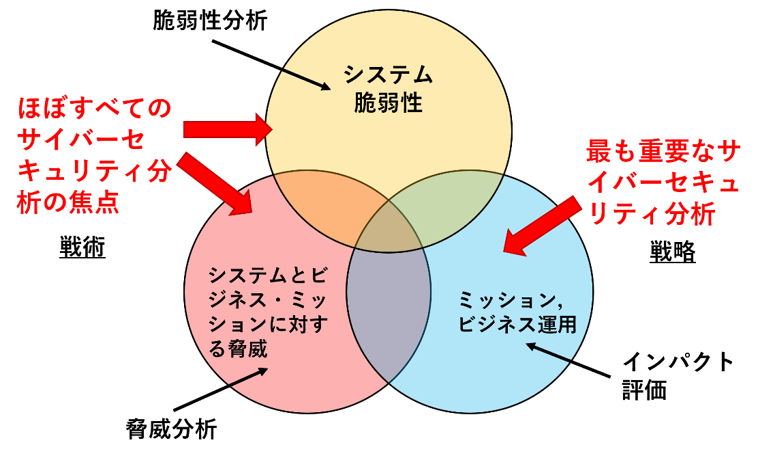
\includegraphics[width=80mm]{safety_assurance_contents/ch3images/fig-3-3-1-01.png}
    \caption[short]{サイバーセキュリティ分析の3つの種類(STPA-Sec2020より引用)}
\end{figure}

STPA-Secの手順は、STPAの手順にいくつかの工程を加えた以下の手順になります。
\begin{itemize}
    \item Step 1 問題設定+分析目的の定義
    \item Step 2 安全制御構造図のモデル化
    \item Step 3 非安全制御動作の識別(Identify Hazard Control Actions)
    \item Step 4 ロスシナリオの識別 + セキュリティシナリオの識別 + ウォーゲーム(Wargaming)
\end{itemize}
%
\begin{figure}[H]
    \centering
    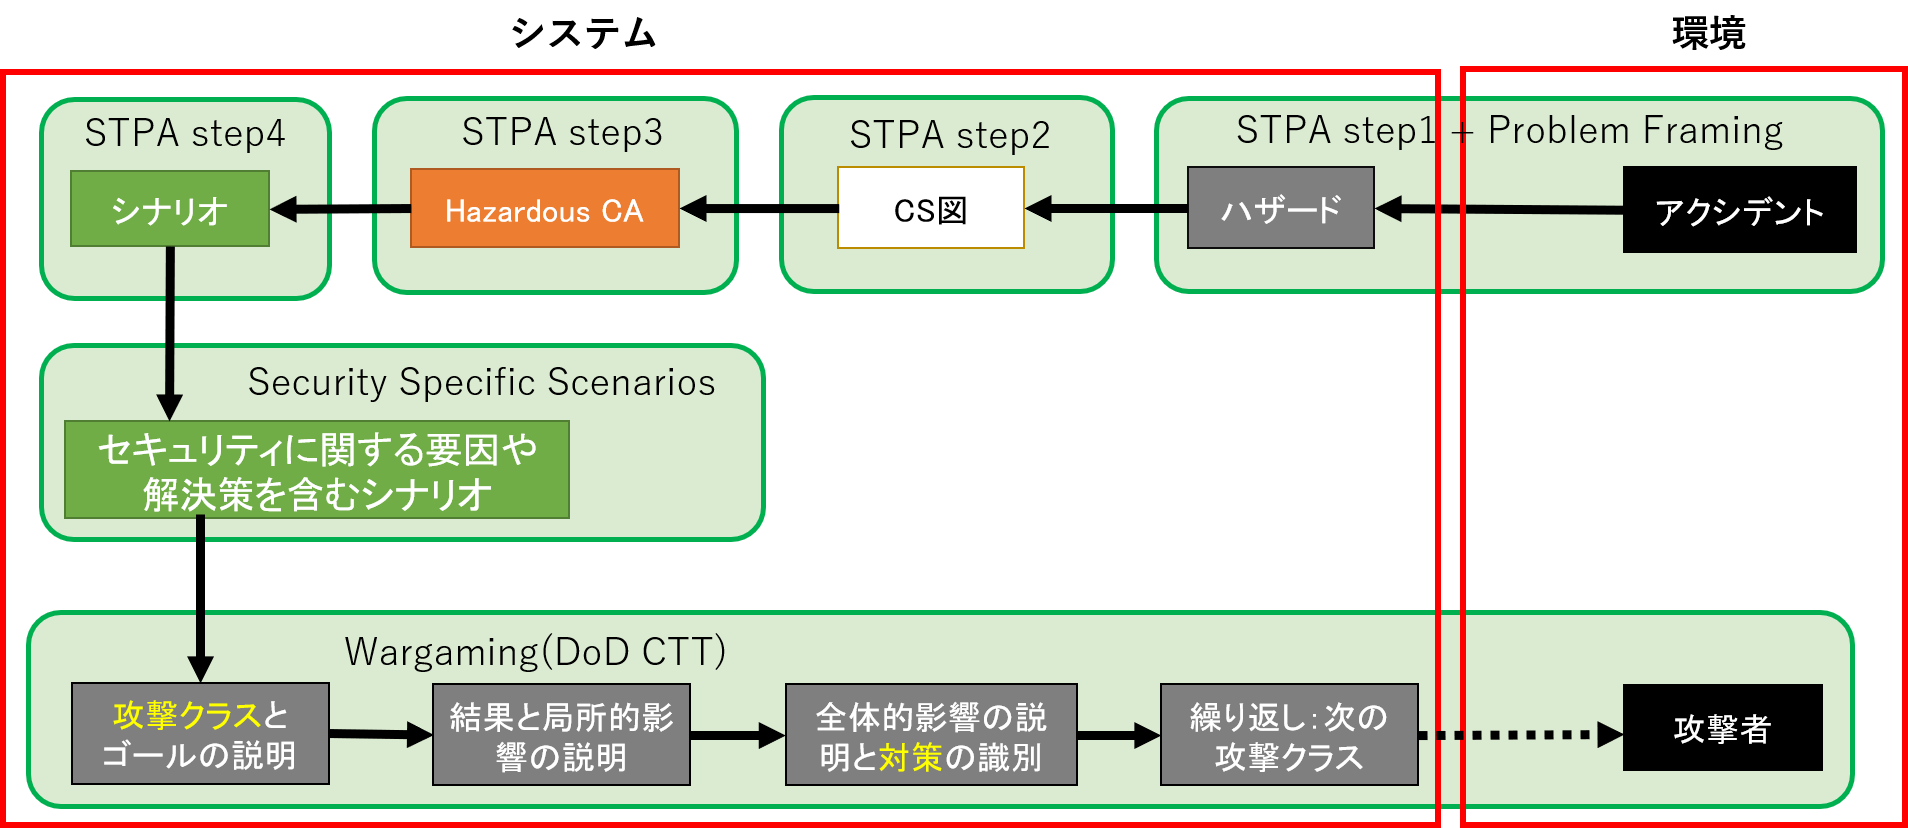
\includegraphics[width=80mm]{safety_assurance_contents/ch3images/fig-3-3-1-02.png}
    \caption[short]{STPA-Sec Wargaming Using DoD Cyber Table Top}
\end{figure}

STPA-Sec Step 1では、問題設定(Problem Framing)に加え、STPA Step 1の分析目的を行います。
STPA Step 1では、安全に関する損失とハザードを識別しますが、STPA-Sec Step 1では、セキュリティに関する損失とハザードも識別します。
例えば、損失として会社の信用が、ハザードとして権限を持たない人が(情報システム内の)個人情報を閲覧可能な状態などがあげられます。

問題設定では、システムが何をすることになっているかを簡潔に説明する文章を構成します。
この文章には、ステークホルダーとの会話と資料から抽出した目的(purpose)、方法(method)、目標(goal)
や制約/制限(Constraints/Restraints)に加え、作成した機能モデル(functional model)の記述が含まれます。
この文章の様式は、
「{Why=目標}に貢献するために、{What=目的}を{How=方法}によって行うシステム。ただし、{While=制約/制限}を満たすこと。」
のようになります。
問題設定で構成する文章の例としては、「Why{制動距離を短くすること}に貢献するために、What{タイヤがロックして滑り始めたら、ブレーキを自動的に緩めること}をHow{ホール速度を計測し、タイヤのロックを検知し、ブレーキ圧力開放を指示(ブレーキ圧力発生を解除)}によって行うシステム。ただし、Where{走行の安全の確保}を行うこと。」等が挙げられます。

STPA-Sec Step 2では、STPA Step 2と同様に安全制御構造図を構築します。
今回は、以下の安全制御構造図を考えることにします。
%
\begin{figure}[H]
    \centering
    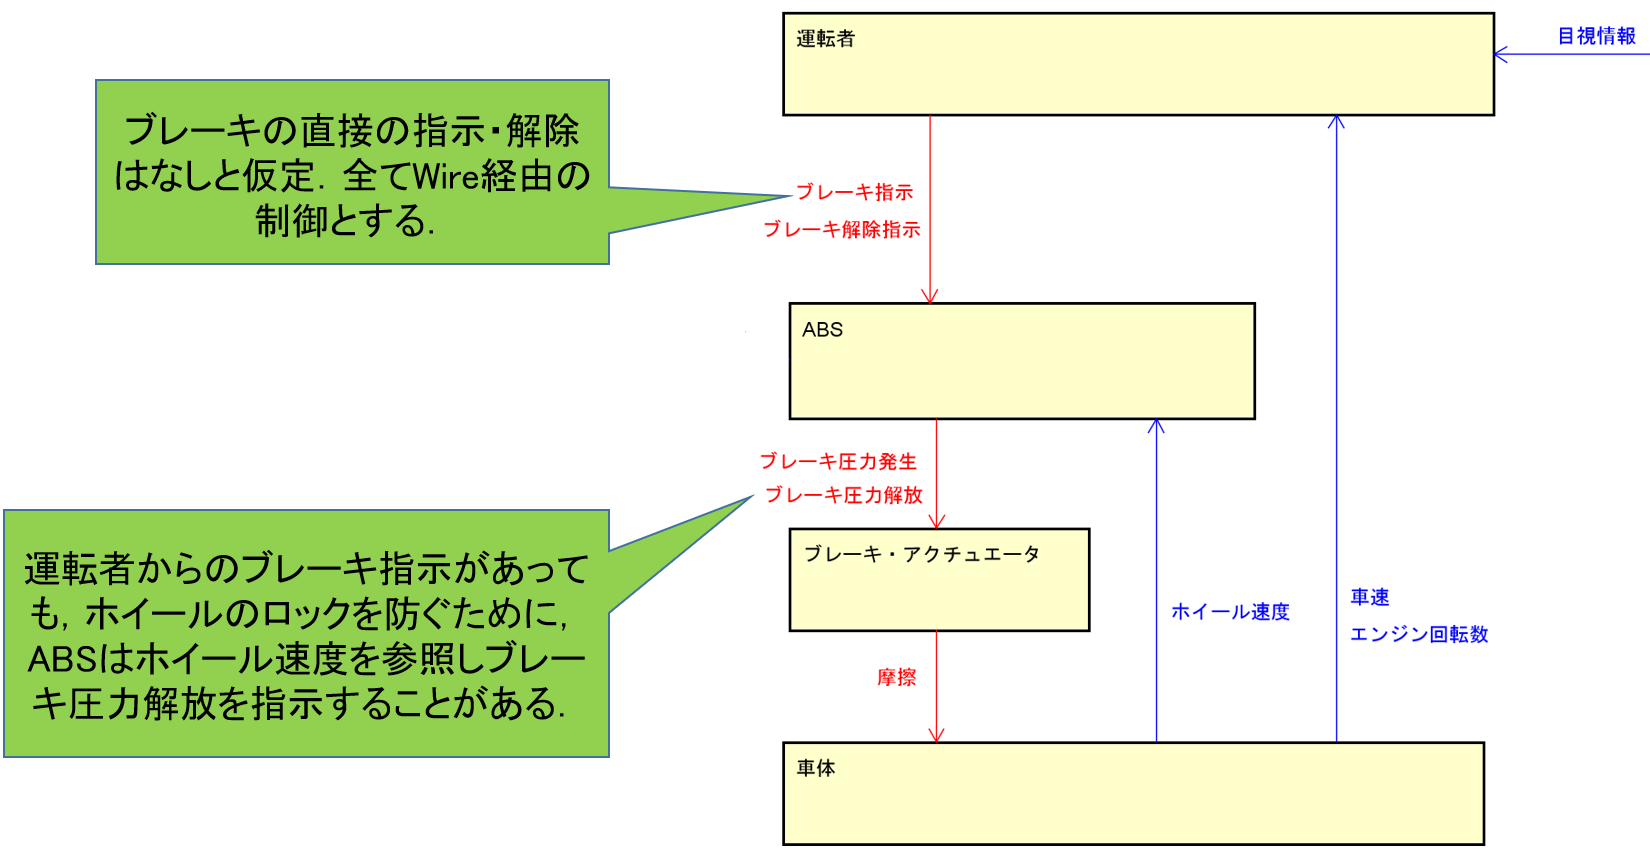
\includegraphics[width=80mm]{safety_assurance_contents/ch3images/fig-3-3-1-03.png}
    \caption[short]{STPA-Secで使用する安全制御構造図の例}
\end{figure}

STPA-Sec Step 3では、STPA Step 3と同様に非安全動作を識別します。
STPAの場合、非安全動作(Unsafe Control Action)という用語を使いましたが、
STPA-Secでは、安全とセキュリティを両方分析するため、Hazardous Control Actionという用語が使われています。
本書では、どちらも非安全動作という訳語としています。

上の図中のコントロールアクション「ブレーキ圧力発生」に対するUCAの例\textcolor{red}{(もっと整合的・現実的な例に置き換えること)}としては、
%
\begin{itemize}
    \item HCA-P1:運転者からのブレーキ指示がないのに、ABSがブレーキ圧力発生を指示してしまい、後続車両に追突される。
    \item HCA-N1:運転者からの指示があるのに、ABSがブレーキ圧力発生を指示しないため、前方障害物に衝突する。
\end{itemize}
%
が考えられます。
次のStepでUCAへ至るシナリオを識別しますが、
HCA-N1に対するシナリオでは、安全要因がUCAを引き起こすかもしれないし、セキュリティ要因がUCAを引き起こすかもしれません。

STPA-Sec Step 4では、STPA Step 4と同様に、ロスシナリオを識別します。
なお、セキュリティに係る要因もロスシナリオに含めるため、セキュリティに係るヒントを追加したり、
コントロールループ図に加え、セキュリティ分析で使用する図も参照すると有効です。

例えば、HCA-N1に対するロスシナリオを識別します。
このとき、プロセスモデルの不一致「ABSがホイール速度を誤認識(ロック状態であると誤認識)」を基に、
ロスシナリオの識別を進めることにします。
なお、プロセスモデルの不一致「ABSがホイール速度を誤認識(ロック状態であると誤認識)」が起こると、
「走行中に、ABSがホイール速度を誤認識(ロック状態であると誤認識)してしまい、
ブレーキ圧力発生を指示せずにブレーキ圧力解放を指示を出して、HCA-N1へ至る」となるため、
プロセスモデルの不一致の要因も識別すれば、ロスシナリオが識別されます。
この誤認識は不適切なコントロールアルゴリズム
「ABSは運転者からのブレーキ指示があり、かつホイール回転速度からロック状態でないと認識しているときには、ブレーキ圧力発生を指示しない」
により引き起こされます。
さらにこの不適切なアルゴリズムが実装された理由としては、
ソフトウェアの動作検証が不十分であることや、外部からの不適切なソフトウェアの更新といったセキュリティ要因が考えられます。

STPA-Sec Step 4では、次にセキュリティシナリオを識別します。
セキュリティシナリオの定義は明確ではありませんが、
「しばしばロスシナリオと同じであるが、セキュリティに関連する原因(cause)と解決策(solution)を含むことがある」
とあることから、ロスシナリオの要因と対策部分としてセキュリティに関連する要因と解決策を識別したシナリオであると考えられます。
既にロスシナリオが識別されているため、ロスシナリオを含むSTPAの分析結果を利用できます。
さらに、セキュリティの分析で利用されている、STRIDEなどの攻撃の分類を用いることで、シナリオの要因部分を識別できます。
セキュリティと安全のかかわり方としては、セキュリティに関する要因が安全を脅かすというシナリオが主に思い浮かびますが、この逆も考えらえます。

例えば、ロスシナリオと同様に、HCA-N1に対するセキュリティシナリオを識別します。
このとき、プロセスモデルの不一致「ABSがホイール速度を誤認識(ロック状態であると誤認識)」を基に、ロスシナリオの識別を進めることにします。
今回は、コントロールアルゴリズムは適切
「ABSは運転者からのブレーキ指示があり、かつホイール回転速度からロック状態でないと認識しているときには、ブレーキ圧力発生を指示する」
であるとします。
しかし走行中に、ABSが誤った入力「ブレーキ解除指示(診断モード)」と「車速は低速」を受信したとします。
するとABSの仕様から、ABSはブレーキ圧力発生を指示せずに、ブレーキ圧力開放を指示してしまい、HCA-N1へ至ります。
またこの誤った入力は、入力の改ざんにより引き起こされます。

%%%%%%%%%%%%%%%%%%%%%%%%%%%%%%%%%%%%%%%%%%%%%%%%%%%%%%%%%%%%%%%%
\subsection{ウォーゲーム(Wargaming)}
%%%%%%%%%%%%%%%%%%%%%%%%%%%%%%%%%%%%%%%%%%%%%%%%%%%%%%%%%%%%%%%%

STPA-Sec Step 4では、最後にウォーゲーム(Wargaming)を実施します。
ウォーゲームの定義は明確ではありませんが、ウォーゲームのDoD Cyber Table Top (CTT)(参考文献)による実施例から、
資産(asset)や侵害されるサイバーセキュリティ・プロパティの識別、攻撃経路(attack path)の分析、攻撃実現性(attack feasibility)の評価を実施していることが分かります。

ウォーゲームでは以下の内容を実施します。
%
\begin{itemize}
    \item STPA-Sec(またはSTPA)で特定されたシナリオを引き起こす攻撃クラスを評価する。
    \item コントロールのクラスの潜在的な有効性を評価する。
    \item 攻撃クラスの実行の複雑さを理解する。
    \item 検討中の機能や特徴に関連する運用リスクの評価をサポートする。
\end{itemize}
%
\begin{figure}[H]
    \centering
    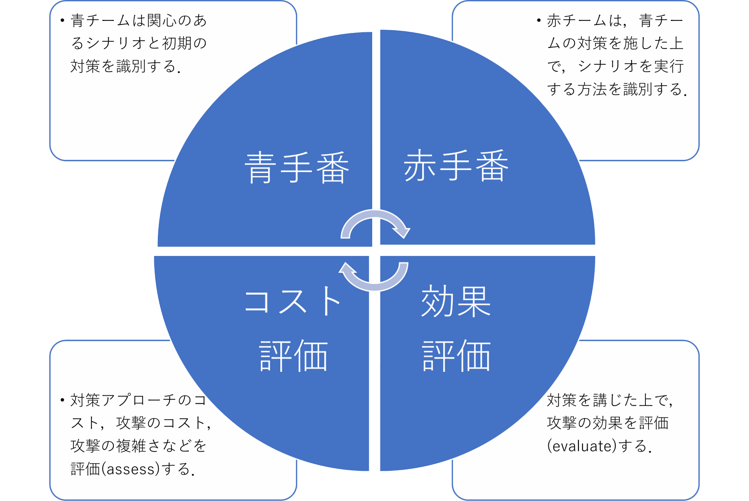
\includegraphics[width=80mm]{safety_assurance_contents/ch3images/fig-3-3-1-04.png}
    \caption{STPA-Sec Wargaming Approach(STPA-Sec2020より引用)}
\end{figure}

これらの内容を実現するための、具体的な手順や作業内容については別の資料を参照することとされています。
ここでは、文献STPA-Secで紹介されているDoD CTT(参考文献)を用いた例を紹介します。
(後ろで参照しやすくするため、各項目にはWG数字の形式で番号を付けることにします)

%%%%%%%%%%%%%%%%%%%%%%%%%%%%%%%%%%%%%%%%%%%%%
\subsubsection{STPA-Sec Wargaming Using DoD Cyber Table Top(CTT)}

\begin{itemize}
    \item WG1:OPFOR(Opposing FORce、仮想敵部隊、赤)が大まかな攻撃クラスとゴールを記述する。
    \item WG2:両チームは成果(outcome)と効果(effect)を記述する。
    \item WG3:作戦チーム(operations team、青)が作戦効果(mission effects)を説明し、回避策(workarounds)を記述する。
    \item WG4:次のクラスの攻撃を繰り返す。
\end{itemize}

さらに、WG1のうち攻撃クラスの記述は以下の項目に細分化され、下線部を識別します。
\begin{itemize}
    \item WG1-1:コントロールストラクチャを検証することで、潜在的な攻撃の大まかな分類についてさらなる洞察が得られる。
    \item WG1-2:攻撃がどの要素(element(s))に\underline{影響}するかを検討・識別する。
        また、\underline{影響を受ける要素(element impacted)}と呼ばれる攻撃が影響する要素を識別する。
    \item WG1-3:STRIDE を使用して、影響を受ける要素に対する攻撃のうち、エフェクト(effect)の原因となるものを識別する。
        (このとき、エフェクトの原因となる攻撃を\underline{攻撃クラス(attack class)}と呼ぶ。)
    \item WG1-4:シナリオに戻り、\underline{攻撃の目的(goal of the attack)}は何かを検討する。
    \item WG1-5:OPFORは「条件なしのHCA」を引き起こしてはならないが、条件が満たされている場合はHCAを引き起こさなければならない。
\end{itemize}

例として、
HCA-N1「運転者からの指示があるのに、ABSが指示を出さないため前方障害物に衝突する」と、
このHCAに対するセキュリティシナリオ「走行中に、ABSが誤ったメッセージ「ブレーキ解除指示(診断モード)」と「車速は低速」を受信したため、
ABSがブレーキ圧力発生を指示せずに、ブレーキ圧力開放を指示して、HCA3-N1へ至る」を考えることにします。
%
\begin{figure}[H]
    \centering
    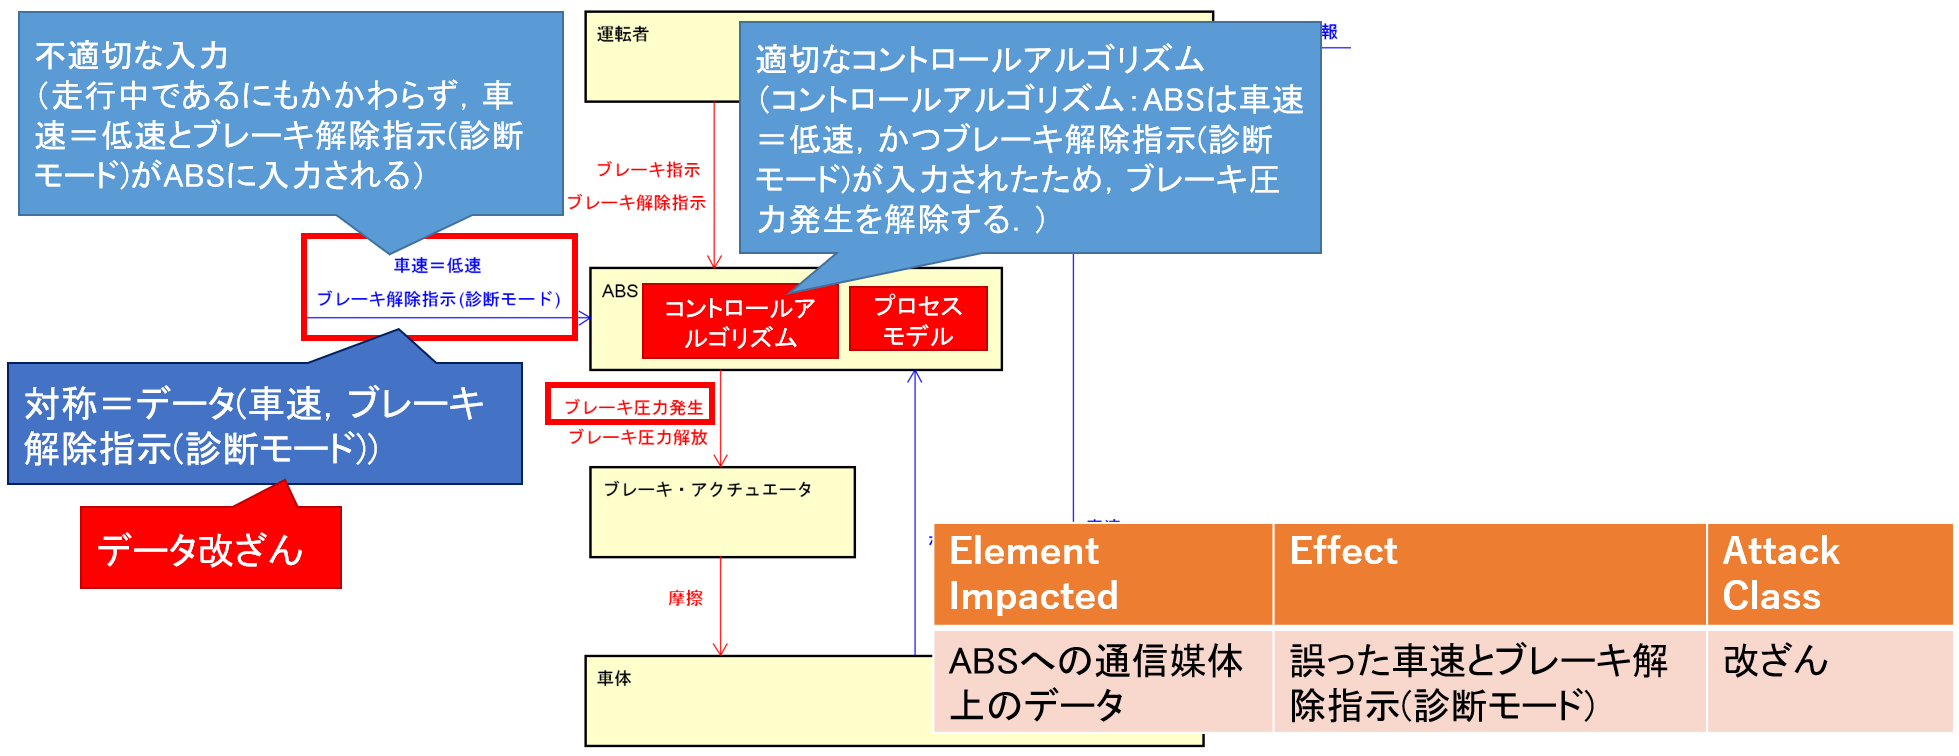
\includegraphics[width=100mm]{safety_assurance_contents/ch3images/fig-3-3-1-05.png}
    \caption{WG1の攻撃クラスの識別の例}
\end{figure}
%
セキュリティシナリオと安全制御構造図から、影響を受ける要素として「ABSへのメッセージ(入力)」が識別され、
このときの影響は「誤ったメッセージ「ブレーキ解除指示(診断モード)」と「車速は低速」」となります。
これらの影響を受ける要素と影響に対し、STRIDEを使用すると、有効な攻撃クラスとして「改ざん」が識別されます。
他方、WG1のゴールの識別では、攻撃成功の条件と攻撃のゴールを識別します。
今回の例では、攻撃成功の条件(コンテキスト)としては「走行中」が識別でき、
攻撃のゴールとしては「ABSがブレーキ指示を出さずにブレーキ解除指示を出す」が識別できます。

WG2では、安全制御構造図に基づいて、攻撃側は「攻撃クラス」を起動するために、いつ「コンテキスト」が成立するかを決定します。
このとき、基本ルール1)制御構造は“土俵(play ground)”である、2)現在の抽象的なレベルにとどまる、
3)前提条件を明示する、4)攻撃側はコンテキスト要件を遵守する、を守るようにします。
今回の例では、攻撃クラス「改ざん」とコンテキスト「走行中」としていたので、
ホイール速度、車速、エンジン回転数から走行中であかどうかを決定できます。

WG3では、作戦チームが攻撃の効果をシステム全体(ミッションレベルまで)で評価し、
回避策(workarounds)を記述する。
攻撃効果の評価には、ロスシナリオ・セキュリティシナリオに対応するハザード・損失を用いることができます。
また、脅威クラスに対処するための4つの大まかな回避策のアプローチとしては、
軽減(mitigate)、排除(eliminate)、転送(transfer)、受け入れる(accept)があります。
なお、回避策を策定する際には、現在の詳細レベルとの一貫性を保つ必要があります。

WG4では、次の攻撃クラスに対しここまでの手順を繰り返します。
今回の例では攻撃クラス「改ざん」を分析したので、例えば、別の攻撃クラス「DoS」を分析します。


% 講義スライドには含まれているが、広義では使っていないので、CASTはスキップします。
%
% %%%%%%%%%%%%%%%%%%%%%%%%%%%%%%%%%%%%%%%%%%%%%%%%%%%%%%%%%%%%%%%%
% \section{CAST(Causal Analysis based on System Theory)}
% %%%%%%%%%%%%%%%%%%%%%%%%%%%%%%%%%%%%%%%%%%%%%%%%%%%%%%%%%%%%%%%%

% CASTは、STAMPに基づく事故分析手法です。実際に発生したアクシデントのシナリオを識別し、システムの安全制御構造がなぜ機能しなかったかを分析します。

% %%%%%%%%%%%%%%%%%%%%%%%%%%%%%%%%%%%%%%%%%%%%%%%%%%%%%%%%%%%%%%%%
% \subsection{CASTの目的}

% CASTの主な目的は以下の通りです:

% \begin{itemize}
%     \item 事故調査の際に問われるべき質問を特定する
%     \item 事故がなぜ起こったのかを明らかにする
%     \item 責任の所在を明らかにするのではなく、システムの改善点を見出す
% \end{itemize}

% %%%%%%%%%%%%%%%%%%%%%%%%%%%%%%%%%%%%%%%%%%%%%%%%%%%%%%%%%%%%%%%%
% \subsection{CASTの手順}

% CASTは以下の手順で実施されます:

% \begin{enumerate}
%     \item 基本情報の収集
%     \item 安全コントロールストラクチャーのモデル化
%     \item 損失における各コンポーネントの分析
%     \item コントロールストラクチャーの欠陥の識別
%     \item 改善プログラムの作成
% \end{enumerate}

%%%%%%%%%%%%%%%%%%%%%%%%%%%%%%%%%%%%%%%%%%%%%%%%%%%%%%%%%%%%%%%%
\section{事例研究: 自動運転システムへのSTPAの適用}
%%%%%%%%%%%%%%%%%%%%%%%%%%%%%%%%%%%%%%%%%%%%%%%%%%%%%%%%%%%%%%%%

\textcolor{red}{ここから再開 2024-09-23}
\textcolor{red}{ページ数的に、国際規格への対応、特にリスク評価の実施について書けばよさげ}
ここでは、自動運転システムにSTPAを適用する例を示します。

%%%%%%%%%%%%%%%%%%%%%%%%%%%%%%%%%%%%%%%%%%%%%%%%%%%%%%%%%%%%%%%%
\subsection{Step 1: 分析目的の定義}

\begin{itemize}
    \item ロス: 人命の損失、車両の損傷
    \item ハザード: 自車両と他の物体(車両、歩行者、障害物など)との距離が安全距離未満になる
    \item 安全制約: 自車両は常に他の物体との安全距離を維持しなければならない
\end{itemize}

%%%%%%%%%%%%%%%%%%%%%%%%%%%%%%%%%%%%%%%%%%%%%%%%%%%%%%%%%%%%%%%%
\subsection{Step 2: 制御構造図のモデル化}

% ここに制御構造図を挿入
\textcolor{red}{[自動運転システムの制御構造図を挿入]}

%%%%%%%%%%%%%%%%%%%%%%%%%%%%%%%%%%%%%%%%%%%%%%%%%%%%%%%%%%%%%%%%
\subsection{Step 3: 非安全制御動作の識別}

UCAの例:
\begin{itemize}
    \item UCA1: 前方に障害物があるにもかかわらず、自動運転システムがブレーキを適用しない
    \item UCA2: 安全な状況下で自動運転システムが不必要にブレーキを適用する
\end{itemize}

%%%%%%%%%%%%%%%%%%%%%%%%%%%%%%%%%%%%%%%%%%%%%%%%%%%%%%%%%%%%%%%%
\subsection{Step 4: ロスシナリオの識別}

ロスシナリオの例:
\begin{itemize}
    \item LS1: センサーの故障により、自動運転システムが前方の障害物を検知できず、ブレーキを適用しない
    \item LS2: ソフトウェアのバグにより、自動運転システムが安全な状況を危険と誤認識し、不必要にブレーキを適用する
\end{itemize}

% CASTは講義で触れていないので、本からも外します。
% %%%%%%%%%%%%%%%%%%%%%%%%%%%%%%%%%%%%%%%%%%%%%%%%%%%%%%%%%%%%%%%%
% \section{事例研究: 鉄道システム事故へのCASTの適用}
% %%%%%%%%%%%%%%%%%%%%%%%%%%%%%%%%%%%%%%%%%%%%%%%%%%%%%%%%%%%%%%%%

% ここでは、実際の鉄道システム事故にCASTを適用する例を示します。

% %%%%%%%%%%%%%%%%%%%%%%%%%%%%%%%%%%%%%%%%%%%%%%%%%%%%%%%%%%%%%%%%
% \subsection{事故概要}

% 2019年6月1日、横浜シーサイドラインの無人自動運転列車が逆走し、終端の車止めに衝突した事故を分析します。

% %%%%%%%%%%%%%%%%%%%%%%%%%%%%%%%%%%%%%%%%%%%%%%%%%%%%%%%%%%%%%%%%
% \subsection{基本情報の収集}

% \begin{itemize}
%     \item 事故日時: 2019年6月1日 20時15分頃
%     \item 場所: 新杉田駅
%     \item 結果: 乗客25名中17名が負傷
%     \item システム: 自動列車運転システム(ATO)、自動列車制御システム(ATC)
% \end{itemize}

% %%%%%%%%%%%%%%%%%%%%%%%%%%%%%%%%%%%%%%%%%%%%%%%%%%%%%%%%%%%%%%%%
% \subsection{安全コントロールストラクチャーのモデル化}

% % ここに安全コントロールストラクチャーの図を挿入
% \textcolor{red}{[鉄道システムの安全コントロールストラクチャー図を挿入]}

% %%%%%%%%%%%%%%%%%%%%%%%%%%%%%%%%%%%%%%%%%%%%%%%%%%%%%%%%%%%%%%%%
% \subsection{各コンポーネントの分析}

% 例: ATOシステムの分析
% \begin{itemize}
%     \item 責任: 列車の自動運転制御
%     \item 不適切な制御行動: 逆方向への出発指示
%     \item 誤ったプロセスモデル: 正しい進行方向の認識の欠如
%     \item コンテキスト: システムの設計上の欠陥
% \end{itemize}

% %%%%%%%%%%%%%%%%%%%%%%%%%%%%%%%%%%%%%%%%%%%%%%%%%%%%%%%%%%%%%%%%
% \subsection{改善提案}

% \begin{itemize}
%     \item ATOシステムの進行方向認識機能の強化
%     \item ATCシステムによる逆走検知機能の改善
%     \item 人間のオペレーターによるバックアップ体制の強化
% \end{itemize}

%%%%%%%%%%%%%%%%%%%%%%%%%%%%%%%%%%%%%%%%%%%%%%%%%%%%%%%%%%%%%%%%
\section{まとめ}
%%%%%%%%%%%%%%%%%%%%%%%%%%%%%%%%%%%%%%%%%%%%%%%%%%%%%%%%%%%%%%%%

STAMP/STPA及びCASTは、現代の複雑なシステムの安全性分析に適した手法です。これらの手法を用いることで、以下のような利点が得られます:

\begin{itemize}
    \item システム全体の安全性を包括的に分析できる
    \item 人間要因を含むシステムの相互作用を考慮できる
    \item 事故の根本原因だけでなく、システムの改善点を特定できる
    \item 設計段階から運用段階まで、システムのライフサイクル全体にわたって適用できる
\end{itemize}

これらの手法を効果的に活用することで、より安全で信頼性の高いシステムの開発と運用が可能になります。

%%%%%%%%%%%%%%%%%%%%%%%%%%%%%%%%%%%%%%%%%%%%%%%%%%%%%%%%%%%%%%%%
\section{参考文献}
%%%%%%%%%%%%%%%%%%%%%%%%%%%%%%%%%%%%%%%%%%%%%%%%%%%%%%%%%%%%%%%%
\begin{itemize}
    \item Engineering a Safer World, 2012
    \item STPA Handbook, 2018
    \item はじめてのSTAMP/STPA, 2016
    \item はじめてのSTAMP/STPA(実践編), 2017
    \item はじめてのSTAMP/STPA(活用編), 2018
    \item STAMPガイドブック ~システム思考による安全分析~, 2019
    \item STAMP Workbench
    \item BASIC INTRODUCTION TO STPA FOR SECURITY (STPA-SEC), 2020 SYSTEM-THEORETIC ACCIDENT MODEL AND PROCESSES (STAMP) WORKSHOP, July 22, 2020, William “Dollar” Young, Jr (Ph D)
    \item System-Theoretic Process Analysis for Security (STPA-SEC): Cyber Security and STPA, WilliamYoung Jr, PhD, 2019 STAMP Conference Boston, MA, March 25, 2019
    \item BASIC INTRODUCTION TO STPA FOR SECURITY (STPA-SEC), 2020 SYSTEM-THEORETIC ACCIDENT MODEL AND PROCESSES (STAMP) WORKSHOP, July 22, 2020, William “Dollar” Young, Jr (PhD) 
    \item System-Theoretic Process Analysis for Security (STPA-SEC): Cyber Security and STPA William Young Jr, PhD Reed Porada 2017 STAMP Conference Boston, MA March 27, 2017
    \item 福島祐子, 「CPSのサイバーセキュリティに求められる安全分析とSTPA-Secの有効性」, ユニシス技報, vol.41,  no.2, Sep.2021
\end{itemize}